\section{Practicality of VRF-based mining}
\label{sec:practicality}

In this section, we experimentally show that VRF-based mining is easy to implement and introduce little overhead.
Our experiment is twofold.
First, we compare the performance of VRFs with three other hash functions used for cryptocurrency mining, namely SHA256D used in Bitcoin, Scrypt used in Litecoin and CryptoNight used in Monero.
The comparison shows that VRF can be much faster than Ethereum and CryptoNight.
Second, we measure the runtime of each step ($H_1$, point multiplication and $H_2$) of $\mathsf{VRFHash}$.
The profiling shows that the point multiplication takes approximately 88\% of $\mathsf{VRFHash}$'s runtime, which is the performance hotspot and can be optimised in the future.

\subsection{Experimental setting}

We implement the standardised EC-VRF in Algorithm~\ref{algo:standard-ecvrf} using Go programming language.
In particular, we use Ed25519~\cite{bernstein2012high} as the underlying elliptic curve, Elligator~\cite{bernstein2013elligator} as $H_1(\cdot)$, SHA-3 as the hash function.
Ed25519, SHA-3 and the encoding of points on Ed25519 are supported by Go's standard library.
We do not apply any optimisations on the EC-VRF implementation.
We use open-source implementations for SHA256D~\ref{github.com/seehuhn/sha256d}, Scrypt~\ref{github.com/elithrar/simple-scrypt}, and CryptoNight~\ref{ekyu.moe/cryptonight}.

All experiments run on a MacBook Pro with a 2.2 GHz Intel Core i7 Processor, a 16 GB DDR4 RAM and 256 SSD storage disk.
For each group of experiment, we run an algorithm for ten times, then take the average data as the experimental results.




\subsection{Comparison between VRF and other mining algorithms}

\begin{figure}[htp]
    \centering
    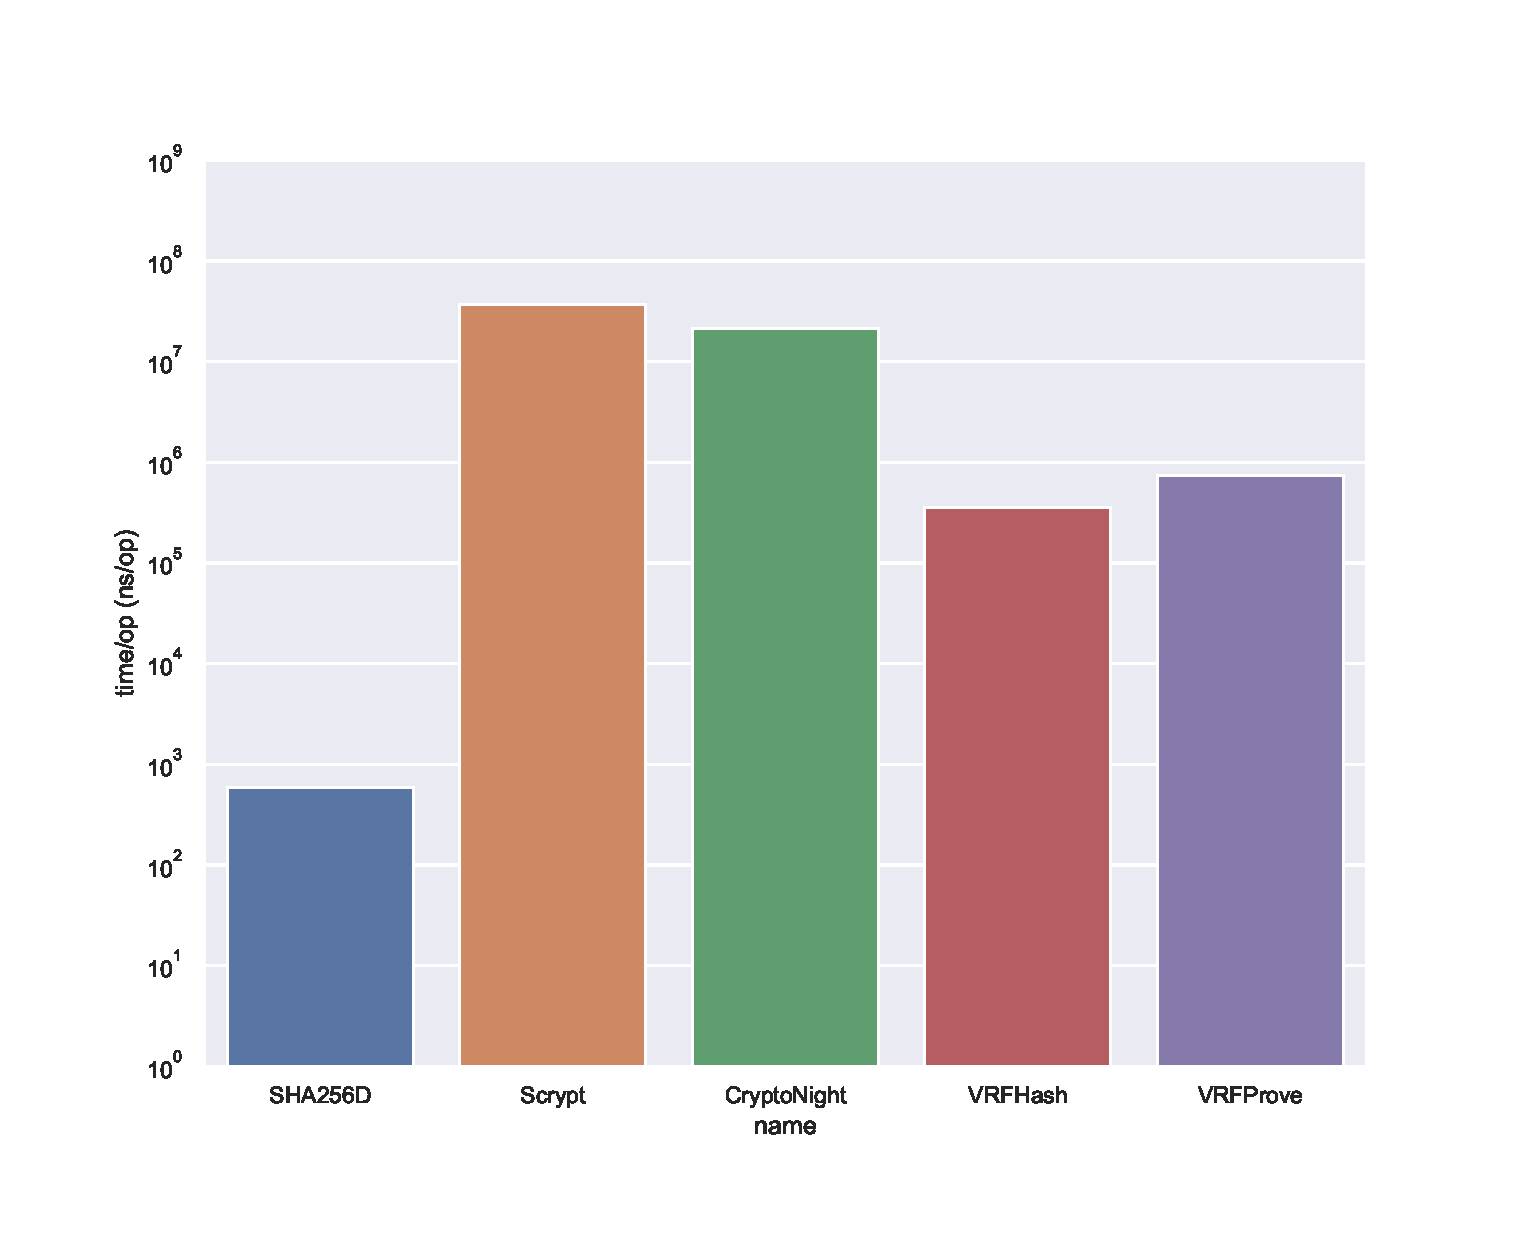
\includegraphics[width=.7\linewidth]{figs/runtime-comparison.eps}
    \caption{Comparing the runtime of VRF and other mining algorithms.}
    \label{fig:runtime-comparison}
\end{figure}

First, we compare the performance of VRF with other mining algorithms.
Figure~\ref{fig:runtime-comparison} shows the runtime of VRF and other algorithms.
First, SHA256D is much faster than other algorithms.
This is because SHA256D is simply executing SHA256 hashing twice, which is quite fast.
Second, $VRFVerify$ is slightly slower than $VRFProve$, and $VRFProve$ is slightly slower than $VRFHash$.
Last, although without optimisation, all functions of VRF are much faster than Scrypt and CryptoNight.
This means that VRF is easy to implement and introduces little overhead, so suitable for cryptocurrency mining.



\subsection{Runtime breakdown of VRF}

Second, we profile $VRFHash$ by evaluating the runtime of its each step.
\TODO{xxx}